\documentclass[12pt,a4paper]{article}
% 文档类:12pt字体,A4纸张,文章类型
\usepackage[margin=1in]{geometry}
% 几何包:设置1英寸边距
\usepackage{graphicx}
% 图形包:插入图片
\usepackage{amsmath}
% AMS数学包:数学公式
\usepackage{amssymb}
% AMS符号包:数学符号
\usepackage{newtxtext,newtxmath} % Times New Roman 字体
% New TX字体包:Times New Roman字体
\usepackage{setspace} % 行距设置
% Setspace包:行距设置
\usepackage{siunitx}
% SI单位包:科学单位
\usepackage[hidelinks]{hyperref} % 去除目录/链接红框
% Hyperref包:超链接,隐藏链接边框
\usepackage{enumitem}
% Enumitem包:列表项
\usepackage{float}
% Float包:浮动环境
\usepackage{subcaption}
% Subcaption包:子标题

% 设置页面格式:1英寸边距,1.5倍行距,12点Times New Roman字体
\geometry{margin=1in}
\onehalfspacing
\setlength{\parindent}{0pt}
\setlength{\parskip}{6pt}

\title{\textbf{EE5112: Human Robot Interaction\\Project 1: Dialogue System and LLM Platform Development}}
% 标题:EE5112:人机交互\\项目1:对话系统和LLM平台开发
\author{Group 7\\
Niu Mu (Matriculation Number)\\
Wu Zining (A0294373W)\\
Zhao Jinqiu (Matriculation Number)}
% 作者:第7组\\
% 牛牧(学号)\\
% 吴子宁(A0294373W)\\
% 赵金秋(学号)
\date{\today}
% 日期:今天

\begin{document}
% 文档开始

\maketitle
% 生成标题页

% 标题页
% Title page with group information and course details

\newpage
% 新页

\tableofcontents
% 生成目录

\newpage
% 新页

% 目录
% Table of contents

\section{Abstract}
% 摘要

% 摘要部分 - 简要概述项目目标、方法、主要发现和结论
% Abstract section - Brief overview of project objectives, methods, key findings and conclusions

[Placeholder for abstract content - 150-250 words]
% [摘要内容占位符 - 150-250字]

% 关键词
% Keywords
\textbf{Keywords:} Dialogue System, LLM, Human-Robot Interaction, Natural Language Processing, TensorFlow
% 关键词:对话系统,LLM,人机交互,自然语言处理,TensorFlow

\section{Introduction}
% 引言

% 引言部分 - 介绍对话系统和LLM的背景,项目目标和意义
% Introduction section - Background of dialogue systems and LLMs, project objectives and significance

\subsection{Background}
% 背景

% 背景介绍 - 对话系统在人机交互中的重要性
% Background introduction - Importance of dialogue systems in human-robot interaction

[Placeholder for background content]
% [背景内容占位符]

\subsection{Project Objectives}
% 项目目标

% 项目目标 - 基于课程要求的具体目标
% Project objectives - Specific objectives based on course requirements

The main objectives of this project are:
% 本项目的主要目标是:
\begin{enumerate}
    \item To familiarize with the process of developing a dialogue system
    % 熟悉对话系统开发过程
    \item To familiarize with the working environment and Python packages
    % 熟悉工作环境和Python包
    \item To familiarize with popular platforms such as TensorFlow
    % 熟悉TensorFlow等流行平台
    \item To familiarize with popular open source LLMs (Llama, GLM, etc.)
    % 熟悉Llama、GLM等流行开源LLM
    \item To develop a dialogue system and local LLM platform
    % 开发对话系统和本地LLM平台
    \item To familiarize with LLM evaluation procedures
    % 熟悉LLM评估程序
    \item To provide practical experience in problem-finding and problem-solving
    % 提供问题发现和解决的实践经验
\end{enumerate}

\subsection{Project Scope}
% 项目范围

% 项目范围 - 定义项目边界和预期贡献
% Project scope - Define project boundaries and expected contributions

[Placeholder for project scope content]
% [项目范围内容占位符]

\section{Task 1: Development Environment Setup}
% 任务1:开发环境搭建

% 任务1:开发环境搭建 - 熟悉Python包、TensorFlow等工具的使用
% Task 1: Development Environment Setup - Familiarize with Python packages, TensorFlow and other tools

\subsection{Python Environment Configuration}
% Python环境配置

% Python环境配置 - 安装和配置必要的Python包
% Python environment configuration - Installation and configuration of necessary Python packages

[Placeholder for Python environment setup content]
% [Python环境设置内容占位符]

\subsection{TensorFlow Platform Familiarization}
% TensorFlow平台熟悉

[Placeholder for TensorFlow familiarization content]
% [TensorFlow熟悉内容占位符]

\subsection{Development Tools and Libraries}
% 开发工具和库

[Placeholder for development tools content]
% [开发工具内容占位符]

\section{Task 2: LLM Platform Development}
% 任务2:LLM平台开发

\subsection{Open Source LLM Exploration}
% 开源LLM探索

% 开源LLM探索 - 研究和测试Llama、GLM等开源LLM
% Open source LLM exploration - Research and test open source LLMs like Llama, GLM

\subsubsection{Literature Review on LLM Categories}
% 不同类型LLM的文献综述


Large Language Models (LLMs) can be categorized into three main architectural paradigms based on their transformer configurations: encoder-decoder, encoder-only, and decoder-only models. Each architecture has distinct characteristics, strengths, and applications in natural language processing tasks.
% 大型语言模型(LLM)可以根据其transformer配置分为三种主要架构范式:编码器-解码器、仅编码器和仅解码器模型。每种架构都有独特的特征、优势和在自然语言处理任务中的应用。

\paragraph{Encoder-Decoder Models}
% 编码器-解码器模型

Encoder-decoder models employ a dual-transformer architecture where the encoder processes input sequences to generate contextual representations, while the decoder generates output sequences based on these representations. This architecture is particularly effective for sequence-to-sequence tasks such as machine translation, text summarization, and question answering.
% 编码器-解码器模型采用双transformer架构,其中编码器处理输入序列以生成上下文表示,而解码器基于这些表示生成输出序列。这种架构特别适用于序列到序列任务,如机器翻译、文本摘要和问答。

\textbf{Key Characteristics:}
% 关键特征:
\begin{itemize}
    \item Bidirectional attention in the encoder captures context from both directions
    % 编码器中的双向注意力从两个方向捕获上下文
    \item Unidirectional attention in the decoder enables autoregressive generation
    % 解码器中的单向注意力实现自回归生成
    \item Explicit separation between understanding (encoding) and generation (decoding) phases
    % 理解(编码)和生成(解码)阶段的明确分离
\end{itemize}

\textbf{Representative Models:}
% 代表性模型:
\begin{itemize}
    \item \textbf{T5 (Text-to-Text Transfer Transformer)}: Treats all NLP tasks as text-to-text problems, achieving state-of-the-art performance across diverse benchmarks
    % T5(文本到文本转换transformer):将所有NLP任务视为文本到文本问题,在各种基准上实现最先进的性能
    \item \textbf{BART (Bidirectional and Auto-Regressive Transformers)}: Combines bidirectional encoder with autoregressive decoder, excelling in text generation and denoising tasks
    % BART(双向和自回归transformer):结合双向编码器和自回归解码器,在文本生成和去噪任务中表现出色
    \item \textbf{mT5}: Multilingual extension of T5 supporting over 100 languages
    % mT5:T5的多语言扩展,支持超过100种语言
\end{itemize}

\paragraph{Encoder-Only Models}
% 仅编码器模型

% 仅编码器模型 - 如BERT、RoBERTa等
% Encoder-only models - such as BERT, RoBERTa, etc.

Encoder-only models utilize only the encoder component of the transformer architecture, employing bidirectional attention to process input sequences. These models excel at understanding and representation learning tasks rather than text generation.
% 仅编码器模型仅使用transformer架构的编码器组件,采用双向注意力来处理输入序列。这些模型擅长理解和表示学习任务,而不是文本生成。

\textbf{Key Characteristics:}
% 关键特征:
\begin{itemize}
    \item Bidirectional attention mechanism captures full context
    % 双向注意力机制捕获完整上下文
    \item Optimized for understanding tasks rather than generation
    % 针对理解任务而非生成进行优化
    \item Require task-specific heads for downstream applications
    % 需要特定于任务的头部用于下游应用
    \item Typically used for classification, named entity recognition, and feature extraction
    % 通常用于分类、命名实体识别和特征提取
\end{itemize}

\textbf{Representative Models:}
% 代表性模型:
\begin{itemize}
    \item \textbf{BERT (Bidirectional Encoder Representations from Transformers)}: Pioneer in bidirectional language modeling, achieving breakthrough performance in NLU tasks
    % BERT(来自transformers的双向编码器表示):双向语言建模的先驱,在NLU任务中实现突破性性能
    \item \textbf{RoBERTa}: Optimized version of BERT with improved training procedures and longer training duration
    % RoBERTa:BERT的优化版本,具有改进的训练程序和更长的训练持续时间
    \item \textbf{DeBERTa}: Enhanced BERT with disentangled attention mechanism and enhanced mask decoder
    % DeBERTa:具有解缠注意力机制和增强掩码解码器的增强BERT
    \item \textbf{ELECTRA}: More efficient pre-training using replaced token detection instead of masked language modeling
    % ELECTRA:使用替换token检测而不是掩码语言建模的更高效预训练
\end{itemize}

\paragraph{Decoder-Only Models}
% 仅解码器模型

% 仅解码器模型 - 如GPT系列、LLaMA等
% Decoder-only models - such as GPT series, LLaMA, etc.

Decoder-only models rely exclusively on the decoder component with causal (unidirectional) attention, making them highly effective for autoregressive text generation tasks. This architecture has become the dominant paradigm for modern conversational AI systems.
% 仅解码器模型完全依赖于具有因果(单向)注意力的解码器组件,使其对自回归文本生成任务非常有效。这种架构已成为现代对话AI系统的主导范式。

\textbf{Key Characteristics:}
% 关键特征:
\begin{itemize}
    \item Unidirectional attention prevents information leakage during training
    % 单向注意力防止训练期间信息泄漏
    \item Optimized for text generation and completion tasks
    % 针对文本生成和完成任务进行优化
    \item Can be fine-tuned for various downstream tasks through instruction following
    % 可以通过指令跟随针对各种下游任务进行微调
    \item Generally require larger model sizes to achieve competitive performance
    % 通常需要更大的模型尺寸来实现竞争性性能
\end{itemize}

\textbf{Representative Models:}
% 代表性模型:
\begin{itemize}
    \item \textbf{GPT (Generative Pre-trained Transformer) Series}: GPT-1, GPT-2, GPT-3, and GPT-4 represent the evolution of decoder-only models with increasing scale and capabilities
    % GPT(生成式预训练transformer)系列:GPT-1、GPT-2、GPT-3和GPT-4代表了仅解码器模型的演变,具有不断增加的规模和能力
    \item \textbf{LLaMA (Large Language Model Meta AI)}: Efficient decoder-only model achieving competitive performance with smaller parameter counts
    % LLaMA(Meta AI大型语言模型):高效的仅解码器模型,以较少的参数计数实现竞争性性能
    \item \textbf{GLM (General Language Model)}: Chinese-developed model combining autoregressive and autoencoding approaches
    % GLM(通用语言模型):中国开发的模型,结合自回归和自编码方法
    \item \textbf{PaLM (Pathways Language Model)}: Google's large-scale decoder-only model with 540B parameters
    % PaLM(Pathways语言模型):谷歌的大型仅解码器模型,具有540B参数
\end{itemize}

\subsubsection{Comparative Analysis}
% 对比分析

% 对比分析 - 不同类型LLM的特点和应用场景
% Comparative analysis - Characteristics and application scenarios of different LLM types

\begin{table}[H]
\centering
\caption{Comparison of LLM Architecture Types}
% LLM架构类型比较
\label{tab:llm_comparison}
\begin{tabular}{|l|l|l|l|}
\hline
\textbf{Aspect} & \textbf{Encoder-Decoder} & \textbf{Encoder-Only} & \textbf{Decoder-Only} \\
% 方面 & 编码器-解码器 & 仅编码器 & 仅解码器
\hline
Primary Use & Seq2Seq tasks & Understanding tasks & Generation tasks \\
% 主要用途 & Seq2Seq任务 & 理解任务 & 生成任务
\hline
Attention Mechanism & Bidirectional + Causal & Bidirectional & Causal \\
% 注意力机制 & 双向 + 因果 & 双向 & 因果
\hline
Training Efficiency & Medium & High & Low (for large models) \\
% 训练效率 & 中等 & 高 & 低(对于大型模型)
\hline
Inference Speed & Medium & Fast & Slow (for large models) \\
% 推理速度 & 中等 & 快 & 慢(对于大型模型)
\hline
Task Flexibility & High & Medium & High \\
% 任务灵活性 & 高 & 中等 & 高
\hline
Parameter Efficiency & Medium & High & Low \\
% 参数效率 & 中等 & 高 & 低
\hline
Representative Models & T5, BART & BERT, RoBERTa & GPT, LLaMA \\
% 代表性模型 & T5, BART & BERT, RoBERTa & GPT, LLaMA
\hline
\end{tabular}
\end{table}

\textbf{Performance Trade-offs:}
% 性能权衡:

\begin{itemize}
    \item \textbf{Encoder-Decoder Models}: Offer balanced performance for both understanding and generation tasks, but require more computational resources due to dual architecture
    % 编码器-解码器模型:为理解和生成任务提供平衡性能,但由于双重架构需要更多计算资源
    \item \textbf{Encoder-Only Models}: Excel at understanding tasks with high efficiency, but limited generation capabilities
    % 仅编码器模型:在理解任务中表现出色且高效,但生成能力有限
    \item \textbf{Decoder-Only Models}: Superior generation quality and conversational abilities, but require significant computational resources for training and inference
    % 仅解码器模型:生成质量和对话能力优越,但训练和推理需要大量计算资源
\end{itemize}

\textbf{Application Scenarios:}
% 应用场景:

\begin{itemize}
    \item \textbf{Encoder-Decoder}: Machine translation, text summarization, question answering systems
    % 编码器-解码器:机器翻译、文本摘要、问答系统
    \item \textbf{Encoder-Only}: Sentiment analysis, named entity recognition, text classification, feature extraction
    % 仅编码器:情感分析、命名实体识别、文本分类、特征提取
    \item \textbf{Decoder-Only}: Conversational AI, creative writing, code generation, instruction following
    % 仅解码器:对话AI、创意写作、代码生成、指令跟随
\end{itemize}

\subsubsection{Recent Trends and Future Directions}
% 最新趋势和未来方向

Recent developments in LLM architectures show several emerging trends:
% LLM架构的最新发展显示出几个新兴趋势:

\begin{itemize}
    \item \textbf{Scale Integration}: Modern models increasingly combine multiple architectural paradigms (e.g., encoder-decoder with decoder-only components)
    % 规模集成:现代模型越来越多地结合多种架构范式(例如,编码器-解码器与仅解码器组件)
    \item \textbf{Efficiency Optimization}: Focus on reducing computational requirements while maintaining performance through techniques like knowledge distillation and model compression
    % 效率优化:通过知识蒸馏和模型压缩等技术减少计算需求同时保持性能
    \item \textbf{Multimodal Integration}: Extension of decoder-only models to handle multiple modalities (text, vision, audio)
    % 多模态集成:扩展仅解码器模型以处理多种模态(文本、视觉、音频)
    \item \textbf{Specialized Architectures}: Development of task-specific architectures optimized for particular domains or applications
    % 专用架构:开发针对特定领域或应用的特定任务架构
\end{itemize}

This comprehensive understanding of different LLM architectures provides the foundation for selecting appropriate models for specific applications in dialogue systems and local LLM platforms.
% 对不同LLM架构的全面理解为在对话系统和本地LLM平台中选择适当模型提供了基础。




% Task 2.2
\subsection{Local LLM Platform Implementation}
% 本地LLM平台实现

This subsection details the design and implementation of our local Large Language Model (LLM) platform developed in Task 2. The platform enables fully offline, multi-turn dialogue with an optimized quantized Llama 3.2 3B Instruct model using the \texttt{llama-cpp-python} backend, supporting streaming token-level generation, context management, and persistent conversation storage.
% 本小节介绍任务2中本地LLM平台的设计与实现。平台基于 \texttt{llama-cpp-python} 运行量化的 Llama 3.2 3B Instruct 模型,支持完全离线、多轮对话、逐 token 流式输出、上下文管理以及对话持久化存储。

\subsubsection*{System Architecture}
% 系统架构

The platform is organized into two core layers: (1) \textbf{LLMPlatform} (model runtime + generation control) and (2) \textbf{DialogueSystem} (session orchestration + persistence). 
% 平台包含两个核心层:(1)\textbf{LLMPlatform}(模型运行时与生成控制),(2)\textbf{DialogueSystem}(会话编排与持久化)。

\begin{itemize}[leftmargin=1.2em]
    \item \textbf{Model Runtime}: Wraps the quantized GGUF model (\texttt{Llama-3.2-3B-Instruct-Q4\_K\_M.gguf}) providing unified load / generate / stream interfaces.  
    % 模型运行时:封装量化GGUF模型,提供统一加载/生成/流式接口。
    \item \textbf{Generation Engine}: Applies sampling controls (temperature, top-p, top-k, repeat penalty) and stop-sequence management for safe termination.  
    % 生成引擎:应用采样控制与停止序列管理。
    \item \textbf{Context Builder}: Dynamically composes an instruction-style prompt with system, user, assistant roles; trims history (sliding window) to remain within \texttt{n\_ctx}.  
    % 上下文构建器:动态组装 system/user/assistant 角色提示,采用滑动窗口裁剪历史。
    \item \textbf{Streaming Layer}: Exposes a Python generator yielding incremental tokens for real-time UX.  
    % 流式层:通过生成器逐 token 产出,实现实时交互体验。
    \item \textbf{Persistence Module}: Serializes conversations to JSON with timestamps and metadata (conversation ID).  
    % 持久化模块:将带时间戳的对话序列化为JSON。
    \item \textbf{Configuration Loader}: Merges external \texttt{config.json} with safe defaults; separates model, generation, dialogue, and hardware domains.  
    % 配置加载器:合并外部配置与默认值,分离模型/生成/对话/硬件四类域。
\end{itemize}

\subsubsection*{Configuration and Parameterization}
% 配置与参数化

Four configuration groups enable reproducibility and hardware-aware tuning (excerpt from \texttt{config.json}).
% 四类配置支持可复现与硬件感知调优(摘自 \texttt{config.json})。

\begin{table}[H]
\centering
\caption{Configuration Groups and Key Parameters}
% 配置分组与关键参数
\label{tab:config_params}
\begin{tabular}{|l|p{0.26\linewidth}|p{0.5\linewidth}|}
\hline
	\textbf{Group} & \textbf{Key Fields} & \textbf{Purpose} \\
% 分组 & 关键字段 & 目的
\hline
Model & model\_path, n\_gpu\_layers, n\_ctx, n\_threads & Load quantized model; balance context length vs memory footprint. \\
Generation & temperature, top\_p, top\_k, repeat\_penalty, max\_tokens & Control diversity, prevent repetition, limit response budget. \\
Dialogue & max\_history, system\_prompt, streaming, save\_conversations & Maintain conversational coherence and UX features. \\
Hardware & gpu\_enabled, max\_gpu\_layers, memory\_fraction & Allocate GPU layers and avoid memory oversubscription. \\
\hline
\end{tabular}
\end{table}

\subsubsection*{Inference Workflow}
% 推理工作流

\begin{enumerate}[leftmargin=1.2em]
    \item \textbf{Initialization}: Validate model presence; instantiate \texttt{Llama} with GPU offloading (\texttt{n\_gpu\_layers=35}).
    % 初始化:验证模型文件,创建 Llama 实例并执行 GPU 分层卸载。
    \item \textbf{Input Capture}: User utterance appended to in-memory history (role-tagged JSON objects).
    % 输入捕获:用户消息追加到内存历史。
    \item \textbf{Context Assembly}: Select last $k$ exchanges (<=6) + system prompt into structured token template.
    % 上下文组装:取最近若干轮 + system prompt 组成结构化模板。
    \item \textbf{Generation}: Call synchronous or streaming API; apply sampling constraints and stop tokens.
    % 生成:同步或流式调用,应用采样与停止序列。
    \item \textbf{Streaming (Optional)}: UI prints incremental tokens; latency perceived as reduced.
    % 流式(可选):界面逐 token 输出,降低感知延迟。
    \item \textbf{Post-processing}: Trim whitespace; append assistant reply to history.
    % 后处理:清理并写回历史。
    \item \textbf{Persistence}: If enabled, serialize pair into conversation JSON (timestamped). 
    % 持久化:若开启,序列化写入 JSON。
\end{enumerate}

\subsubsection*{Streaming Mechanism}
% 流式机制

The streaming interface wraps the backend iterator, yielding \emph{delta} fragments; the UI layer concatenates them to form the final assistant turn. This improves responsiveness for longer generations and mirrors modern production chat UX. A termination check monitors \texttt{finish\_reason} in the final chunk.
% 流式接口封装底层迭代器,逐步输出增量文本分片,界面拼接形成完整回复;提升长回答交互响应性,并监测最后块的 \texttt{finish\_reason} 实现有序终止。

\subsubsection*{Data Persistence and Reproducibility}
% 数据持久化与可复现性

Conversations are stored under \texttt{conversations/} using ISO8601 timestamps for auditing. Each file aggregates ordered message tuples preserving role, content, and creation time, enabling later evaluation or fine-tuning dataset curation.
% 对话以 ISO8601 时间戳文件名保存在 \texttt{conversations/},保留角色/内容/时间顺序,便于评估与后续数据蒸馏或微调语料整理。

\subsubsection*{Performance Considerations}
% 性能考量

We adopt Q4\_K\_M quantization to balance memory (\(~3\,GB GPU usage\)) and quality for a consumer-grade 16GB GPU. Streaming reduces perceived latency; selective history truncation prevents context overflow. CPU threads (\texttt{n\_threads=8}) parallelize token probability computation for non-offloaded layers.
% 采用 Q4\_K\_M 量化在 16GB GPU 上平衡显存(约3GB)与质量;流式降低感知延迟;历史截断避免上下文溢出;CPU 多线程加速未下放层计算。

\subsubsection*{Reliability and Error Handling}
% 可靠性与错误处理

Model load failures (missing file / incompatible quantization) are trapped with fallback messaging. Generation exceptions during streaming yield an inline error token without aborting the application. Conversation save errors are gracefully warned (non-fatal).
% 模型加载失败(缺文件/量化不兼容)被捕获;流式生成异常以内联错误标记返回;保存失败仅告警而不终止主循环。

\subsubsection*{Strengths and Limitations}
% 优势与局限

\begin{itemize}[leftmargin=1.2em]
    \item \textbf{Strengths}: Offline privacy; modular layering; streaming UX; clean JSON audit trail; hardware-aware configuration.
    % 优势:离线隐私;模块分层;流式体验;JSON 审计轨迹;硬件感知配置。
    \item \textbf{Limitations}: Single-model runtime (no dynamic model pool); absence of advanced memory (vector retrieval); limited evaluation hooks in current phase.
    % 局限:单模型运行;缺向量检索记忆;当前阶段缺少评估挂钩。
    \item \textbf{Future Work}: Add retrieval-augmented generation, multi-model routing, automated quality metrics, and GUI integration.
    % 未来工作:加入检索增强、多模型路由、自动化质量指标与 GUI 集成。
\end{itemize}

\subsubsection*{User Interaction Example}
% 用户交互示例

Figure~\ref{fig:llama_chat_screenshot} shows a real dialogue example captured from the streaming session.
% 图~\ref{fig:llama_chat_screenshot} 展示一次真实流式对话示例。

\begin{figure}[H]
    \centering
    % 注意:若编译器无法处理中文文件名,可将图片重命名为 llama_chat.png 并更新路径。
    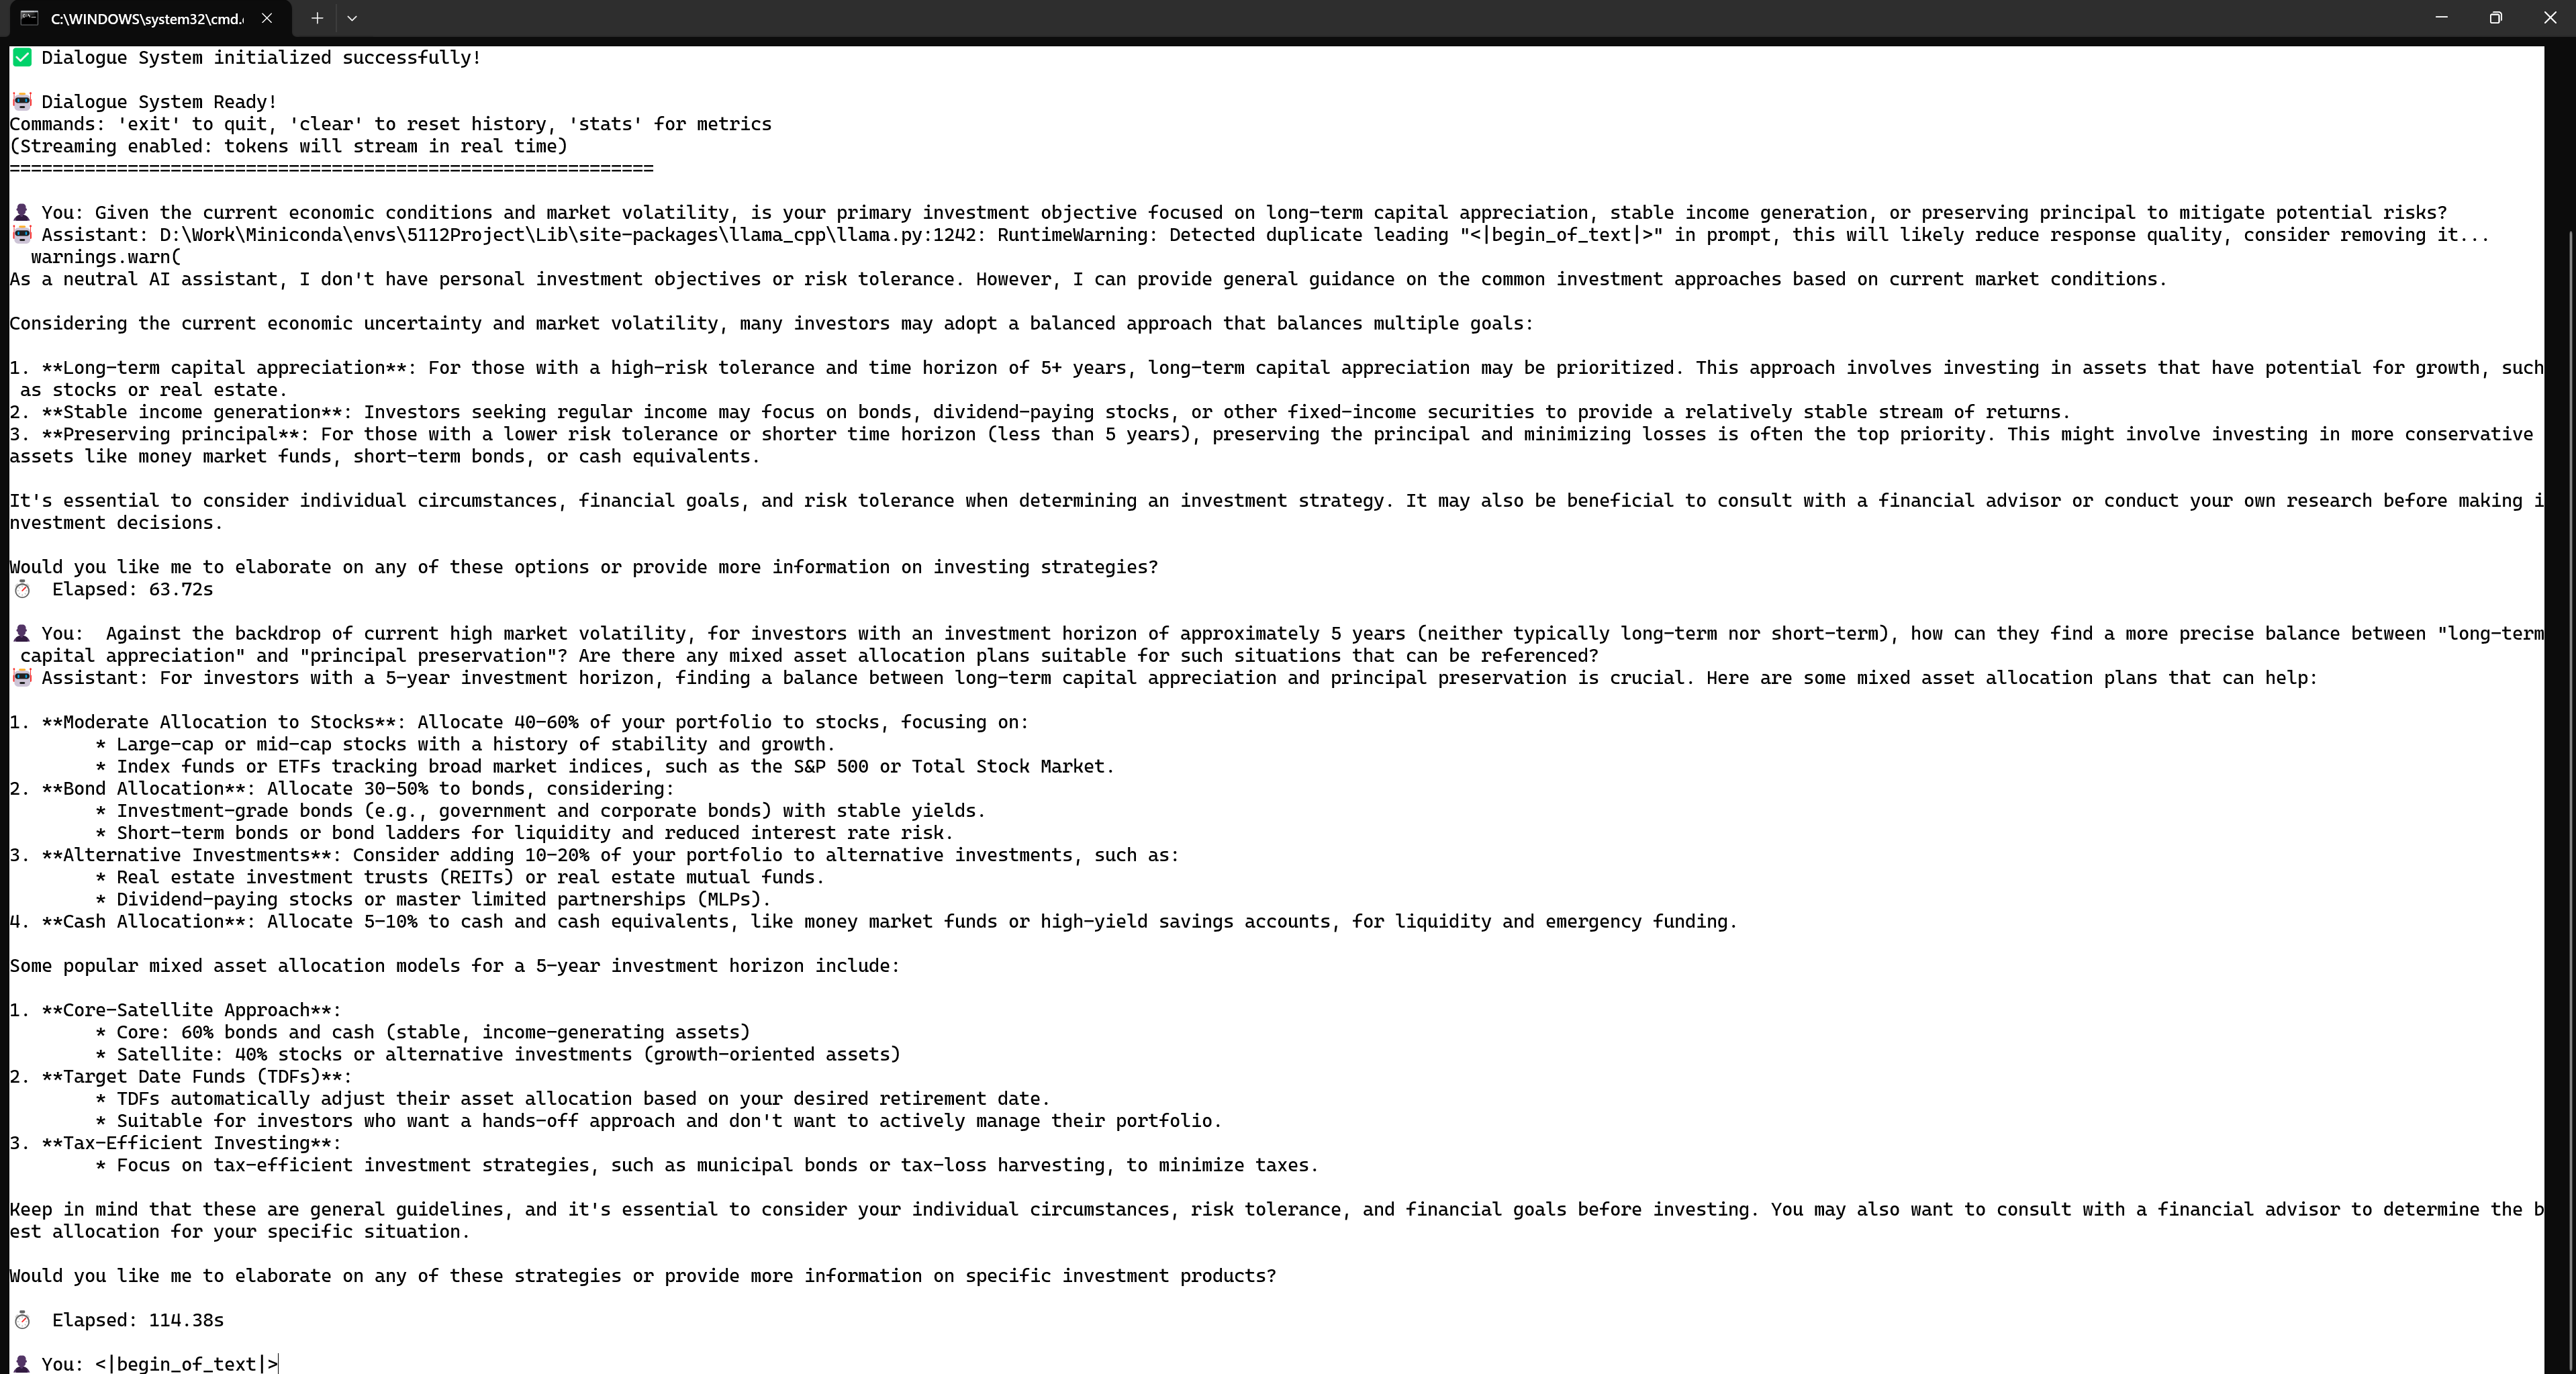
\includegraphics[width=1\linewidth]{Figures/llama对话.png}
    \caption{Example streaming dialogue with local Llama 3.2 3B model.}
    % 使用本地 Llama 3.2 3B 模型的流式对话示例
    \label{fig:llama_chat_screenshot}
\end{figure}

Overall, the implementation delivers a privacy-preserving, extensible inference substrate suitable for subsequent integration with higher-level dialogue management and evaluation modules in later tasks.
% 总体而言,该实现提供一个隐私友好、可扩展的推理底座,为后续任务中的高层对话管理与评估模块集成奠定基础。

\subsection{Comparation of Different Pretrained Models}
% 不同预训练模型的比较

% 本节将对比不同的预训练模型在对话系统中的表现,包括它们的架构、训练数据和生成能力等方面。

\section{Task 3: Dialogue System Development}
% 任务3:对话系统开发

% 任务3:对话系统开发 - 开发完整的对话系统
% Task 3: Dialogue System Development - Develop complete dialogue system

\subsection{Dialogue System Architecture}
% 对话系统架构

% 对话系统架构 - 设计对话系统的整体架构
% Dialogue system architecture - Design overall architecture of dialogue system

[Placeholder for dialogue system architecture content]
% [对话系统架构内容占位符]

\subsection{Natural Language Processing Components}
% 自然语言处理组件

% 自然语言处理组件 - 实现NLP相关功能
% Natural language processing components - Implement NLP-related functions

[Placeholder for NLP components content]
% [NLP组件内容占位符]

\subsection{Multi-modal Communication}
% 多模态通信

% 多模态通信 - 实现文本、语音、图形等多模态交互
% Multi-modal communication - Implement multi-modal interaction including text, speech, graphics

[Placeholder for multi-modal communication content]
% [多模态通信内容占位符]

\subsection{Dialogue Management}
% 对话管理

% 对话管理 - 实现对话状态管理和上下文处理
% Dialogue management - Implement dialogue state management and context processing

[Placeholder for dialogue management content]
% [对话管理内容占位符]

\section{Task 4: System Integration and Testing}
% 任务4:系统集成和测试

% 任务4:系统集成和测试 - 整合所有组件并进行测试
% Task 4: System Integration and Testing - Integrate all components and perform testing

\subsection{Component Integration}
% 组件集成

% 组件集成 - 将LLM平台和对话系统集成
% Component integration - Integrate LLM platform with dialogue system

[Placeholder for component integration content]
% [组件集成内容占位符]

\subsection{System Testing}
% 系统测试

% 系统测试 - 测试整个系统的功能
% System testing - Test overall system functionality

[Placeholder for system testing content]
% [系统测试内容占位符]

\subsection{Performance Optimization}
% 性能优化

% 性能优化 - 优化系统性能
% Performance optimization - Optimize system performance

[Placeholder for performance optimization content]
% [性能优化内容占位符]

\section{Task 5: LLM Evaluation}
% 任务5:LLM评估

% 任务5:LLM评估 - 熟悉LLM评估程序
% Task 5: LLM Evaluation - Familiarize with LLM evaluation procedures

\subsection{Evaluation Metrics}
% 评估指标

% 评估指标 - 定义和选择LLM评估指标
% Evaluation metrics - Define and select LLM evaluation metrics

[Placeholder for evaluation metrics content]
% [评估指标内容占位符]

\subsection{Evaluation Framework Implementation}
% 评估框架实现

% 评估框架实现 - 实现LLM评估框架
% Evaluation framework implementation - Implement LLM evaluation framework

[Placeholder for evaluation framework implementation content]
% [评估框架实现内容占位符]

\subsection{Performance Analysis}
% 性能分析

% 性能分析 - 分析LLM和对话系统的性能
% Performance analysis - Analyze performance of LLM and dialogue system

[Placeholder for performance analysis content]
% [性能分析内容占位符]


\subsection{Solution Implementation}
% 解决方案实现

% 解决方案实现 - 针对挑战的具体解决方案
% Solution implementation - Specific solutions to challenges

[Placeholder for solution implementation content]
% [解决方案实现内容占位符]

\subsection{Code Documentation}
% 代码文档

% 代码文档 - 项目代码的文档化
% Code documentation - Documentation of project code

[Placeholder for code documentation content]
% [代码文档内容占位符]

\section{Results and Discussion}
% 结果和讨论

% 结果和讨论 - 对项目成果的深入讨论和分析
% Results and discussion - In-depth discussion and analysis of project outcomes

\subsection{System Performance Results}
% 系统性能结果

% 系统性能结果 - 展示系统测试结果
% System performance results - Present system testing results

[Placeholder for system performance results content]
% [系统性能结果内容占位符]

\subsection{Task Achievement Summary}
% 任务完成情况总结

% 任务完成情况总结 - 总结各任务的完成情况
% Task achievement summary - Summary of completion status for each task

[Placeholder for task achievement summary content]
% [任务完成情况总结内容占位符]

\subsection{Lessons Learned}
% 经验教训

% 经验教训 - 从项目中学到的经验
% Lessons learned - Experiences gained from the project

[Placeholder for lessons learned content]
% [经验教训内容占位符]

\section{Individual Contributions}
% 个人贡献

% 个人贡献 - 每个组员的个人贡献说明
% Individual contributions - Individual contribution statements for each group member

\subsection{Member 1: Niu Mu}
% 组员1:牛牧

% 组员1:牛牧 - 个人贡献说明
% Member 1: Niu Mu - Individual contribution statement

[Placeholder for Niu Mu's contributions]
% [牛牧贡献占位符]

\subsection{Member 2: Wu Zining (A0294373W)}
% 组员2:吴子宁

% 组员2:吴子宁 - 个人贡献说明
% Member 2: Wu Zining - Individual contribution statement

[Placeholder for Wu Zining's contributions]
% [吴子宁贡献占位符]

\subsection{Member 3: Zhao Jinqiu}
% 组员3:赵金秋

% 组员3:赵金秋 - 个人贡献说明
% Member 3: Zhao Jinqiu - Individual contribution statement

[Placeholder for Zhao Jinqiu's contributions]
% [赵金秋贡献占位符]

\section{Conclusion}
% 结论

% 结论 - 总结项目成果和贡献
% Conclusion - Summary of project outcomes and contributions

\subsection{Project Objectives Achievement}
% 项目目标达成情况

% 项目目标达成情况 - 总结项目目标的完成情况
% Project objectives achievement - Summary of project objective completion

[Placeholder for project objectives achievement content]
% [项目目标达成情况内容占位符]

\subsection{Future Work}
% 未来工作

% 未来工作 - 可能的改进方向
% Future work - Possible directions for improvement

[Placeholder for future work content]
% [未来工作内容占位符]

\section{References}
% 参考文献

% 参考文献 - 引用所有相关文献
% References - Cite all relevant literature

[Placeholder for references - Use proper citation format]
% [参考文献占位符 - 使用正确的引用格式]

\section{Appendix}
% 附录

% 附录 - 补充材料如代码片段、配置文件等
% Appendix - Supplementary materials such as code snippets, configuration files, etc.

\subsection{Code Documentation}
% 代码文档

% 代码文档 - 主要代码片段的文档
% Code documentation - Documentation of main code snippets

[Placeholder for code documentation]
% [代码文档占位符]

\subsection{Configuration Files}
% 配置文件

% 配置文件 - 系统配置文件
% Configuration files - System configuration files

[Placeholder for configuration files]
% [配置文件占位符]

\subsection{User Manual}
% 用户手册

% 用户手册 - 系统使用说明
% User manual - System usage instructions

[Placeholder for user manual]
% [用户手册占位符]

\end{document}
% 文档结束
